\documentclass{article}
\usepackage{graphics}
\usepackage{graphicx}
\usepackage[T1]{fontenc}
\title{CS 742 Foundations of Network Security and Cryptography \\ Assignment 2}
\author{ Ajay Kedare   \space \space 153059007\\ Astha Jada \space \space 153050027 \\ Neha Garg \space \space \space  153050039}
\begin{document}
\maketitle
\clearpage

\section{Computing SHA-1}
\subsection{I (a) Using OpenSSL, compute the SHA-1 hash of a message. Show the output.
Next change a single bit in the message and show the output. What differences
do you observe? Comment on your observations.}

Following steps were followed for computing SHA-1 of the message using openssl:\\

	
\noindent For computing SHA-1 of the message, we created a file of size 1 byte containing only zeroes using following command:\\
\textbf{ dd if=/dev/zero of=binary.dat count=1 bs=1}\\

\noindent The above command created a file binary.dat containing 8 bits of zeros.\\

\noindent The SHA-1 of the message was then computed as shown in figure\\

\noindent Using a hex editor 'bless' we then edited binary.dat that now contains 01 (in hex) in binary i.e we changed only 1 bit. The SHA-1 was then recomputed as shown in figure\\

\noindent It can be observed that eventhough only 1 bit was changed the SHA-1 of the message was changed completely providing more security in a way that one cannot be obtained even if other is already known.
 
 


\section{Computing MAC}
\subsection{I(b) Use OpenSSL to}
\subsubsection{(i) compute the CBC MAC of a message} 
\subsubsection{(ii) verify the CBC MAC on that message}
\subsubsection{(iii) compute the hash MAC of a message}
\subsubsection{(iv) verify the hash MAC on that message}
\subsubsection{(v) sign a message}
\subsubsection{(vi) verify a signature on that message}

\section{Baby Step,Giant Step}
\subsection{II Use the "Baby Step, Giant Step” Algorithm discussed in class to crack the
Discrete Logarithm problem. Your program should input p (the prime number), g
(the generator) and y (the integer whose discrete log is desired) and output x
(the discrete log). Use different sizes for p (8, 10, 12, 14, 16, 18, 20 . . . bits).
For each size of p, use different values of y and plot the average execution time
versus p (log plot).}

\section{XSS attack vectors for DVWA}
\subsection{III Create your own XSS attack vector(s) for DVWA at each security level - low,
medium and high. Investigate why each attack vector works or fails at the
different security levels. Both, persistent and non-persistent (reflected) XSS
attacks should be attempted.}
\textbf{Persistent XSS} : Persistent XSS occurs when the developer stores the user input data into database server
or simply writing it in a file without a proper filtration , then sending them again to the client
browser.\\
\textbf{Reflected XSS} : The non-persistent (or reflected) cross-site scripting vulnerability is by far the
most common type. These holes show up when the data provided by a web client, most commonly
in HTTP query parameters or in HTML form submissions, is used immediately by server-side scripts
to generate a page of results for that user, without properly sanitizing the request.\\
\subsection{Persistent XSS-Level Low}
We'll first change the dvwa security to low.After setting the level click on XSS stored( present on left side).A page will open having name , message textbox along with 'sign guestbook' button. We can enter below attack vectors in name and message textbox.\\
Name: User\\
Message: <script> alert("hi")</script>\\
When user clicks on 'sign guestbook' button, a alert popup box will appear having message 'hi'.\\
cat /var/www/html/dvwa/vulnerabilities/xss\_s/source/low.php-This command is used to get the code of xss stored for low level.\\
Reason for working of attack vector: The two parameters “message” and “name” present in the code  are not sanitized properly.We store these
parameters into the guestbook table, So when we displaying these parameters back the client browser,
it will execute the malicious JavaScript code.\\
\textbf{Stealing cookies}\\
 We can enter below attack vectors in name and message textbox.\\
Name: User\\
Message: <script>alert(document.cookie)</script>\\
When user clicks on 'sign guestbook' button,below alert popup box will appear.\\
\begin{figure}[htb]
		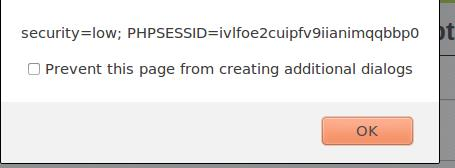
\includegraphics[width=8cm,height=2cm]{cookies.jpg}
		\caption{Computing SHA-1 of the message}
	\end{figure}

Copy this PHPSESSID from the alertbox and save it in a file.This is our cookie and now we have to consume it.There is an add-on for the Mozilla browser titled cookie editor. It is a tool that will let us view the cookies as well as allow us to  edit them.\\
On second machine we'll open the DVWA login page. Now open the cookie editor and search for localhost and we will see the below image
\begin{figure}[htb]
		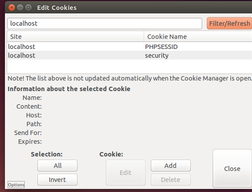
\includegraphics[width=10cm,height=4cm]{cookieeditor.png}
		\caption{Computing SHA-1 of the message}
	\end{figure}
First we'll edit the PHPSESSID cookie and paste the cookie which we have copied earlier in the content textbox. Then we'll modify the security cookie and set the value as low in content textbox and save the changes.Now we'll remove the "login.php" from the URL address and when we press enter we'll be able to login into the dvwa site without providing any credentials.
\subsection{Persistent XSS-Level Medium}
We'll first change the dvwa security to medium.After setting the level click on XSS stored( present on left side).We can enter any one of the  below attack vectors in name textbox. But the size of any input text in name textbox can't be more than 10 characters (maxlength=10), so using firebug we can change the maxlength=80 and then we can enter the below scripts.\\
<script language="javascript">alert("Hi")</script>\\
<scrip<script>t> alert("hi")</script>\\
<SCRIPT> alert('hi');</SCRIPT>\\
In name textbox we can't write <script> keyword directly as the code is replacing <script> keyword with ''(null string).So we have modified the attack vectors accordingly.
In message textbox attack using above scripts will not work because in code message is sanitized by htmlspecialchars(), which will converts some predefined characters to HTML entities.\\
cat /var/www/html/dvwa/vulnerabilities/xss\_s/source/medium.php-This command is used to get the code of xss stored for medium level.\\

\textbf{Stealing cookies}\\
We can steal the cookie in the same way as we did for Persistent XSS-Level Low. But now our attack vector will be in below form and need to put it in name textbox.\\
<SCRIPT>alert(document.cookie)</SCRIPT>\\
While modifying  the security cookie we'll set the value as medium in content textbox. Rest steps of cookie stealing are same as Persistent XSS-Level Low cookie stealing.
\subsection{Persistent XSS-Level High}
We'll first change the dvwa security to high.The “High” level is the secure considered level (it is supposed to be the secure version and not to be passed to teach the secure implementation of web applications for developers).

\subsection{Reflected XSS-Level Low}
We'll first change the dvwa security to low.After setting the level click on XSS Reflected( present on left side).A page will open having a textbox and 'submit' button. We can enter below attack vectors in the textbox.\\
<script> alert('hi');</script>\\
<SCRIPT> alert('hi');</SCRIPT>\\
cat /var/www/html/dvwa/vulnerabilities/xss\_r/source/low.php--This command is used to get the code of xss Reflected for low level.\\
The code is directly echoing the input entered in the textbox without any filtering and sanitization.\\
\textbf{Stealing cookies}\\
We can steal the cookie in the same way as we did for Persistent XSS-Level Low. But here we'll enter the attack vector in the textbox available rather than the message texbox, rest of the steps are same.

\subsection{Reflected XSS-Level Medium}
We'll first change the dvwa security to medium.After setting the level click on XSS Reflected( present on left side).A page will open having a textbox and 'submit' button. We can enter below attack vectors in the textbox.\\
<script language="javascript">alert("Hi")</script>\\
<scrip<script>t> alert("hi")</script>\\
<SCRIPT> alert('hi');</SCRIPT>\\
In the textbox we can't write <script> keyword directly as the code is replacing <script> keyword with ''(null string).So we have modified the attack vectors accordingly.
cat /var/www/html/dvwa/vulnerabilities/xss\_r/source/medium.php--This command is used to get the code of xss Reflected for medium level.\\
The code is directly echoing the input entered in the textbox after replacing <script> keyword with ''(null string). .\\
\textbf{Stealing cookies}\\
We can steal the cookie in the same way as we did for Persistent XSS-Level Medium. But here we'll enter the attack vector in the textbox available rather than the name texbox, rest of the steps are same.
\subsection{Reflected XSS-Level High}
We'll first change the dvwa security to high.The “High” level is the secure considered level (it is supposed to be the secure version and not to be passed to teach the secure implementation of web applications for developers).

\section{SQL Injection}
\subsection{(Level 1) Add yourself as a user with your own username and password providing your IITB roll number in details.}
\subsection{(Level 2) Find out the username-password pairs of ALL the users of this portal.}
\subsection{(Level 3) Find out names of all the tables in the database.}



\end{document}

